\documentclass[a4paper, 12pt]{article}
\usepackage[utf8]{inputenc}
\usepackage[italian]{babel}
\usepackage{titlesec}
\usepackage{graphicx}
\usepackage[ruled,vlined]{algorithm2e}
\usepackage{algorithmic}

\titleformat*{\section}{\LARGE\bfseries}
\titleformat*{\subsection}{\Large\bfseries}
\titleformat*{\subsubsection}{\large\bfseries}
\titleformat*{\paragraph}{\large\bfseries}
\titleformat*{\subparagraph}{\large\bfseries}

\title{Gestione delle stringhe: Tries}
\author{Nicolas Nucifora - X81000452\\\\Università degli studi di Catania\\ Dipartimento di Matematica e Informatica\\\\Algoritmi e laboratorio - Prof. D.F.Santamaria}
\date{A.A 2020/2021}

\begin{document}
\maketitle
\large
\flushleft
\clearpage

\tableofcontents

\clearpage

\section*{Prefazione}
Lo scopo della relazione è analizzare, sotto ogni aspetto, la struttura dati per la gestione delle stringhe chiamata "Trie". Verrà data una sostanziosa descrizione della struttura dati: com'è nata, quali problemi risolve, la sua struttura, come funziona, i pro e i contro del loro utilizzo, e cosi via. Successivamente, si analizzerà lo pseudocodice per l'implementazione delle operazioni per la gestione di un Trie. Infine, il diagramma UML dell'approccio scelto per l'implementazione.
La relazione verrà accompagnata dal codice, scritto in C++, che implementa la struttura, proponendo la risoluzione di uno dei problemi descritti.

\clearpage

\section{Trie: cos'è?}
Il problema di immagazzinare un insieme di parole, come un dizionario con le relative descrizioni o l'insieme delle parole più ricercate su Google, utilizzando poco spazio e la cui ricerca sia molto veloce è uno dei problemi più importanti nel mondo informatico.

Esistono diverse soluzioni, ognuno con i suoi pro e i suoi contro in termini di complessità spaziale e temporale. Un esempio sono le tabelle hash e i dizionari. 

Ma esiste una specifica struttura dati nata appositamente per risolvere il problema della rappresentazione di un insieme di parole: la struttura dati \textbf{Trie}

Il loro utilizzo è stato suggerito per la prima volta dal francese \textbf{René de la Briandais} nel 1959.

La parola "Trie" deriva da re\textbf{trie}val (recupero), in quanto permette di recuperare una parola in pochissimo tempo. 
\vspace{5mm}

Sostanzialmente, un Trie è una struttura ad albero n-ario (il nome trie serve inoltre a distinguerlo da altre strutture ad albero). Ciò che lo differenzia dalle altre strutture ad albero è il fatto che ogni nodo memorizza dentro di se l'intero alfabeto che vogliamo rappresentare (per esempio, 26 lettere per l'alfabeto anglosassone). Strutturando i nodi in modo particolare, è possibile recuperare (re\textbf{trie}ve) una parola/stringa attraversando verso il basso un ramo dell'albero.
\vspace{5mm}

Ma che forma ha un Trie?

\clearpage
\begin{figure}[ht!]
    \centering
    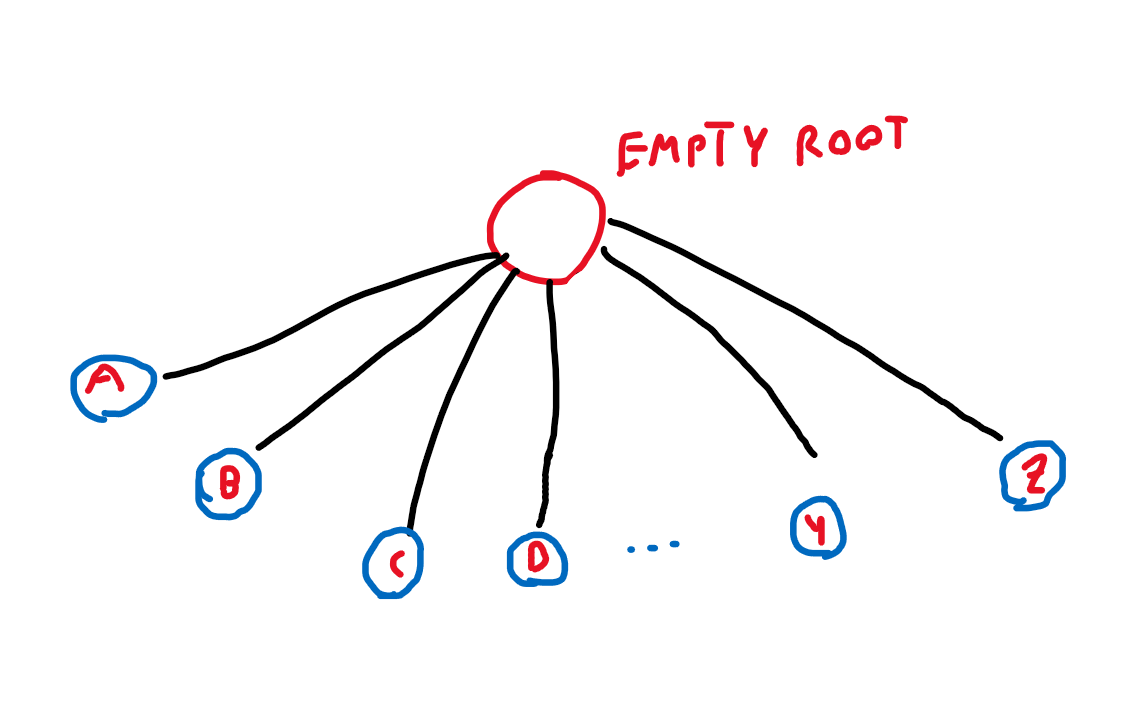
\includegraphics[width=10cm]{Images/shape trie.png}
    \caption{Forma base di un Trie}
    \label{fig:my_label}
\end{figure}

Ogni Trie inizia con un nodo radice vuoto. Esso mantiene dei riferimenti (o link) ai suoi nodi figli, uno per ogni possibile lettera dell'alfabeto. A loro volta, ogni nodo figlio mantiene ulteriori riferimenti alle lettere dell'alfabeto. Questo ci permette di stabilire che \textbf{la dimensione di un Trie è direttamente proporzionale alla grandezza dell'alfabeto che vogliamo rappresentare}.

Per esempio, se l'alfabeto rappresentato è quello anglosassone, ogni nodo mantiene 26 riferimenti alle 26 lettere dell'alfabeto. Mentre, se l'alfabeto rappresentato è \textbf{Khmer}, il numero di riferimenti a nodi figlo che un unico nodo manterrà sarà 74.

Quindi, un Trie potrà essere molto piccolo o molto grande. E' possibile mantenere i riferimenti ai nodi figlo in un Trie in diversi modi, ognuno con i suoi pro e i suoi contro in termini di efficienza spaziale o temporale. Ma per spiegare più nel dettaglio come è strutturato un Trie e come è possibile mantenere e recuperare una stringa da essa, verrà utilizzato l'alfabeto anglosassone, mantenuto attraverso l'utilizzo di un array, il metodo più semplice per implementarlo.

\clearpage
\subsection{Struttura di un Trie}
Ogni nodo, compresa la radice, mantiene due informazioni:
\begin{itemize}
    \item Un valore: che può essere \textbf{NULL}
    \item Un array di riferimenti a nodi figlio: che potrebbero essere \textbf{NULL}
\end{itemize}

\begin{figure}[ht!]
    \centering
    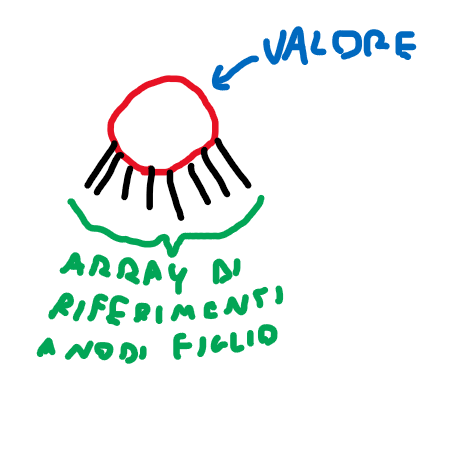
\includegraphics[width=5cm]{Images/nodo trie.png}
    \caption{Nodo di un Trie}
    \label{fig:my_label}
\end{figure}

Quando un Trie viene creato, all'inizio sarà presente solamente il nodo radice. Esso rappresenta la \textbf{stringa vuota}. Il suo valore iniziale sarà \textbf{NULL}. Inoltre, manterrà un array di 26 link ai suoi nodi figlio, che inizialmente avranno valore \textbf{NULL}.

Ogni qualvolta verranno inserite delle stringhe, tali riferimenti verranno riempiti con dei puntatori alle successive lettere che compongono la parola. L'inserimento e come il Trie prende forma verrà spiegato in seguito.

Il motivo della scelta di un array come struttura dati per il mantenimento dei riferimenti è dovuto alla sua semplicità e soprattutto per la velocità di accesso ad ogni cella (in tempo costante). Infatti, se l'alfabeto viene rappresentato in ordine, possiamo associare ad ogni indice dell'array una lettera dell'alfabeto: \textbf{0} per la lettera \textbf{A}, \textbf{1} per la lettera \textbf{B}, e cosi via, fino ad arrivare a \textbf{25} per la lettera \textbf{Z}.

Successivamente, verranno messi a confronto \textbf{Trie} e \textbf{Tabella hash} per mostrare perchè è conveniente utilizzare la prima per mantenere un set di parole.

Nel paragrafo successivo, verrà mostrato come riempire un Trie e come funziona la ricerca di una parola.

\subsection{Costruire un Trie}
Nella figura seguente è mostrato un esempio di un Trie riempito con le seguenti parole: \textbf{Algoritmo, Amazon, Astronauta, Asterix, Sogno}.

\begin{figure}[ht!]
    \centering
    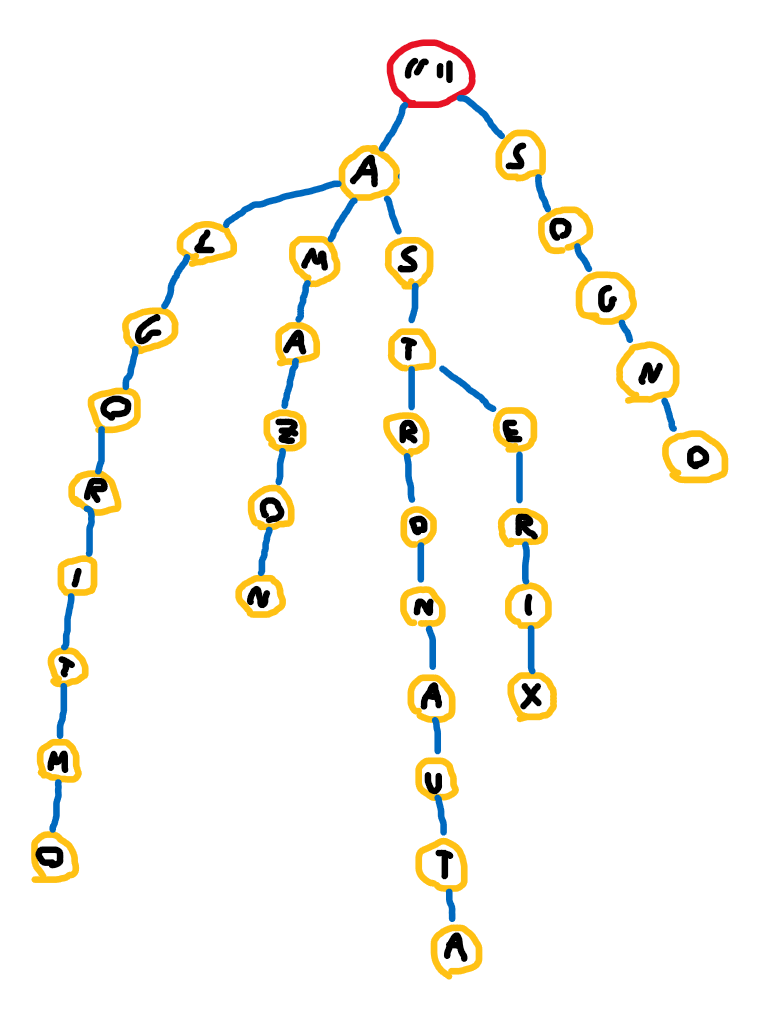
\includegraphics[width=8cm]{Images/esempio trie riempitp.png}
    \caption{Esempio di un Trie riempito}
    \label{fig:my_label}
\end{figure}

Per semplicità, non sono stati mostrati i nodi NULL, ovverro che non contengono riferimenti ad altre lettere.

Come è gia stato spiegato, il nodo radice rappresenta la stringa vuota. Dei suoi 26 riferimenti, l'indice \textbf{0} mantiene un puntatore ad un nodo figlio, in questo caso il puntatore al nodo \textbf{A}, mentre la cella di indice \textbf{18} mantiene un riferimento al nodo \textbf{S}. Tutti gli altri nodi sono \textbf{NULL}.

Ci sono in totale cinque rami, uno per ogni parola rappresentata. Tutte le parole, tranne \textbf{Sogno}, condividono il nodo \textbf{A}, mentre altre parole condividono più nodi. In questo esempio, \textbf{Astronauta} e \textbf{Asterix} condividono i nodi \textbf{A}, \textbf{S} e \textbf{T}.

\subsection{Operazioni}
Ma come si inserisce/cerca/elimina una parola?
\subsubsection{Inserimento}
Vogliamo inserire una nuova parola nella struttura: \textbf{"Amazzone"}.

Per farlo, dobbiamo:
\begin{itemize}
    \item Verificare che la parola non esista già nel Trie, esplorando i nodi.
    \item Se non esiste, riempire i riferimenti ai nodi figlio dove le lettere della parola dovrebbero stare.
\end{itemize}

Ma come facciamo a sapere se una parola esiste o meno?

Abbiamo detto che ogni nodo, oltre ai riferimenti ai nodi figlio, mantiene anche un valore. Tale valore può avere qualunque forma: un valore alfanumerico, una struttura dati, o semplicemente un booleano. Quel valore, se non è \textbf{NULL}, rappresenta \textbf{la fine della stringa}. Quindi, se una parola esiste, la sua ultima lettera, ovvero il suo ultimo nodo, avrà un valore diverso da \textbf{NULL}.

Prendendo come esempio la parola \textbf{Amazzone}, descriviamo passo per passo l'inserimento di una nuova parola:

\begin{itemize}

    \item Partendo dalla radice, controlliamo se il riferimento alla lettera \textbf{A} è presente, essendo la prima lettera che compone la parola \textbf{Amazzone}.
    
    \item Il riferimento al nodo \textbf{A} è diverso da \textbf{NULL}, quindi è presente. Scendiamo verso il basso scandendo le successive lettere che compongono \textbf{Amazzone}: \textbf{A-M-A-Z}.
    
    \item La prossima lettera da controllare è la seconda \textbf{Z} di \textbf{Amazzone}. Il primo nodo \textbf{Z} (che dal principio compone la parola \textbf{Amazon}) non ha un riferimento ad una seconda \textbf{Z}, infatti è \textbf{NULL}. Possiamo creare un nuovo nodo e inserire il suo riferimento alla cella 25 dell'array mantenuto dalla prima lettera \textbf{Z}.
    
    \item Incontreremo ulteriori link \textbf{NULL} anche per le successive lettere \textbf{O}, \textbf{N} ed \textbf{E}. Non faremo altro che creare nuovi nodi e posizionare i riferimenti rispettivamente nelle celle: \textbf{O = 14} (nel secondo nodo \textbf{Z}), \textbf{N = 13} (nel nodo \textbf{O} appena inserito), \textbf{E = 4} (nel nodo \textbf{N} creato subito dopo).
    
    \item Infine, essendo \textbf{E} l'ultima lettera della parola \textbf{Amazzone}, per indicare che questo nodo rappresenta la fine della parola, inseriamo un valore diverso da NULL (in questo esempio \textbf{25}). Se avessimo utilizzato un booleano, bastava settarlo a \textbf{TRUE}.
    
\end{itemize}

\clearpage
\begin{figure}
    \centering
    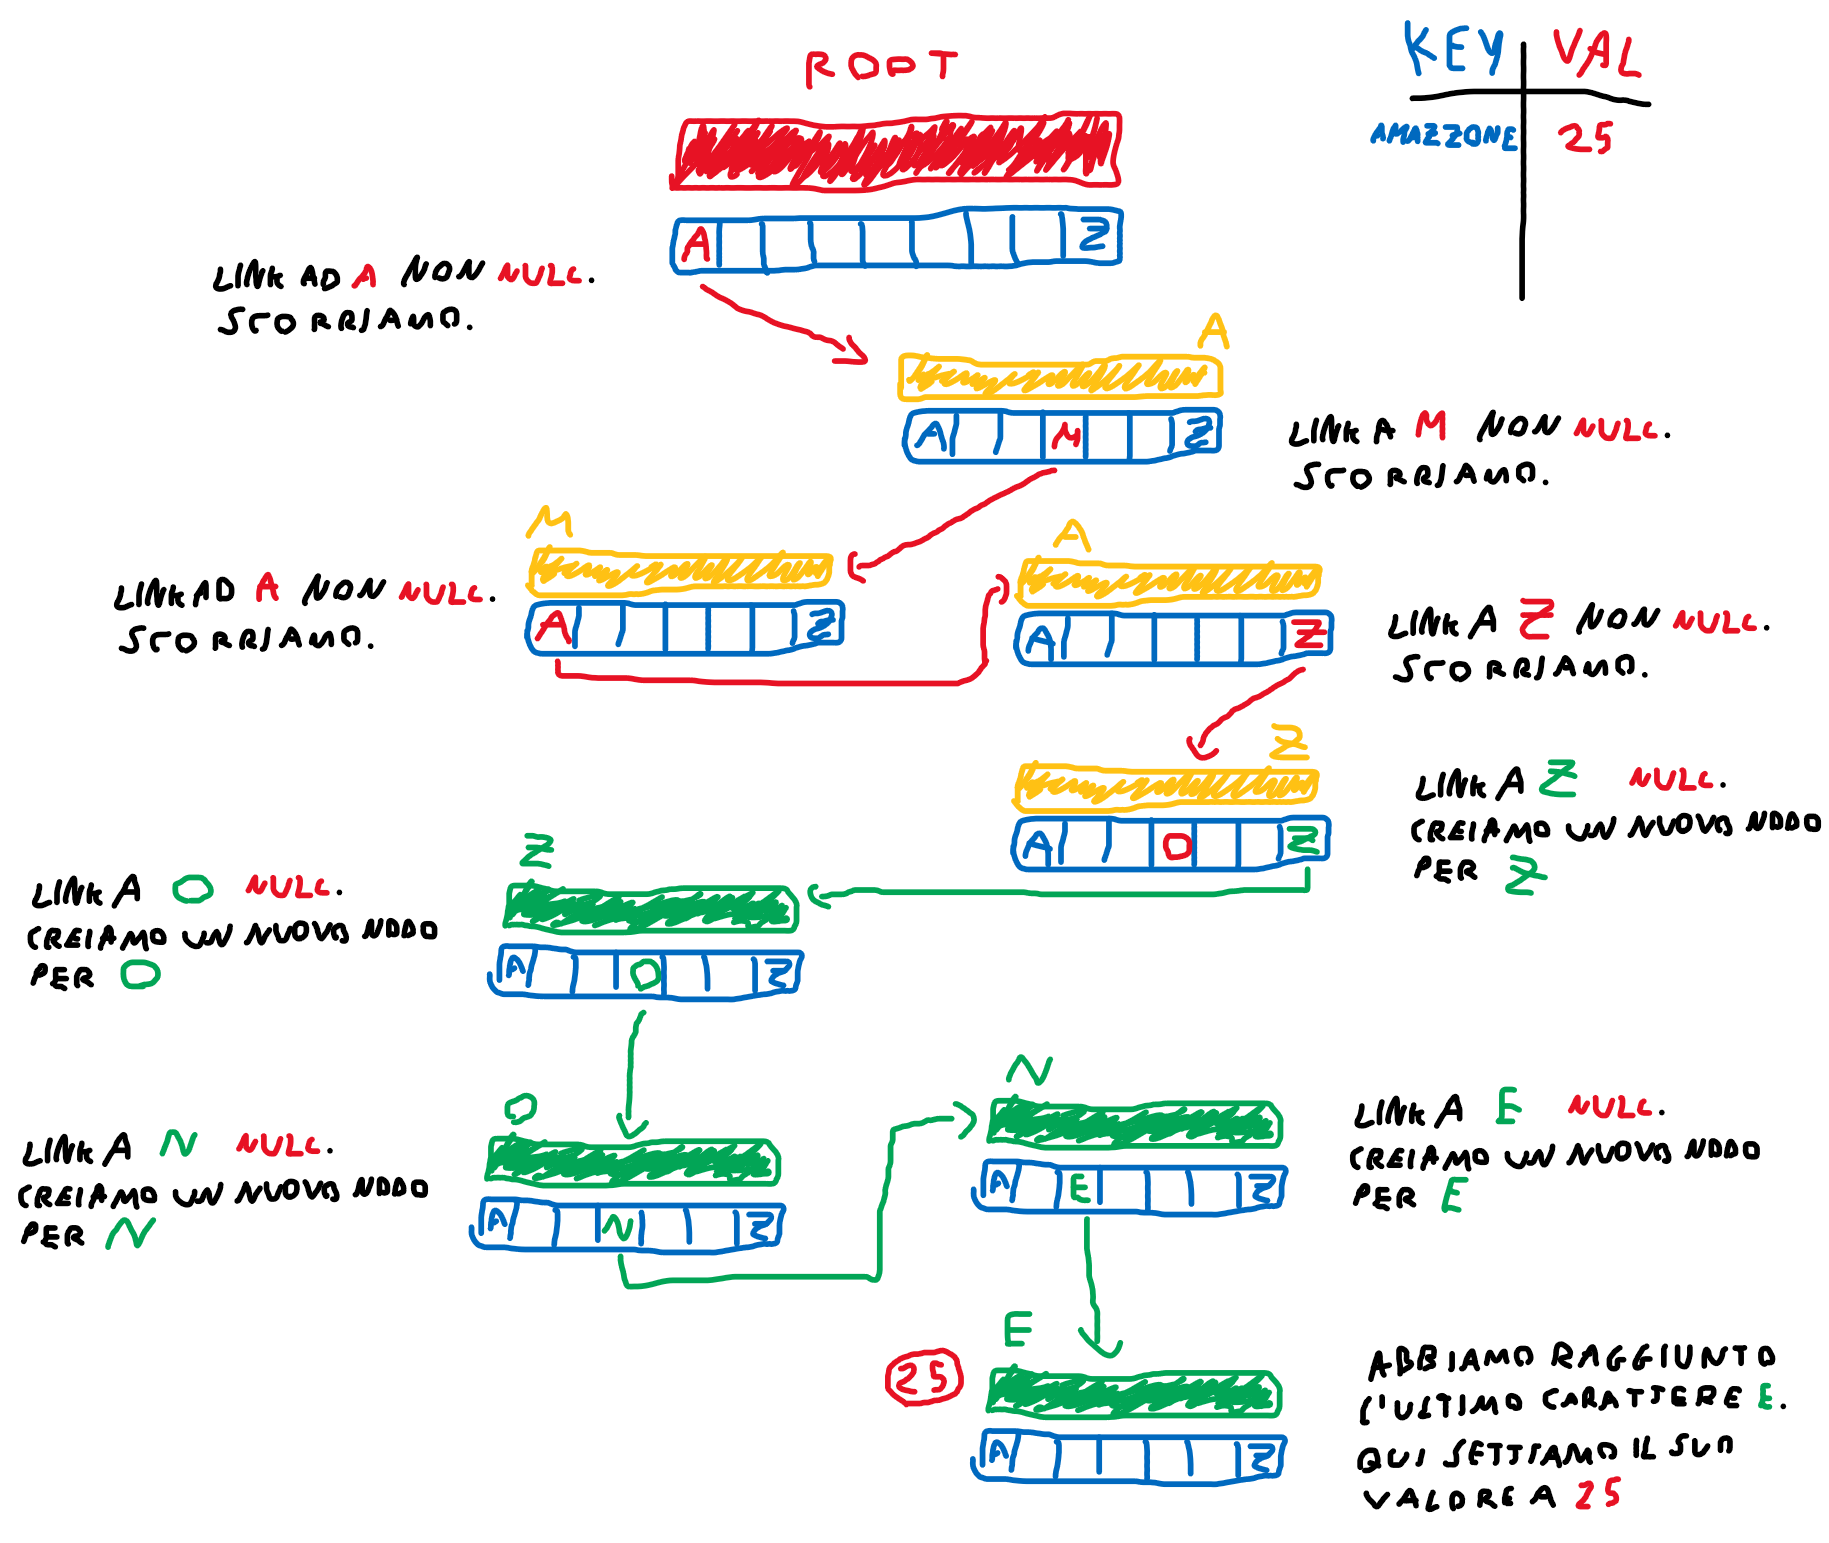
\includegraphics[width=13cm]{Images/esempio inserimento.png}
    \caption{Esempio di inserimento "Amazzone"}
    \label{fig:my_label}
\end{figure}

\clearpage

E se volessimo inserire il prefisso \textbf{Astro} della parola \textbf{Astronauta}? I nodi \textbf{A - S - T - R - O} sono gia stati creati grazie all'inserimento della parola \textbf{Astronauta}. Quindi, per poter inserire \textbf{Astro} nel set delle parole del Trie, basta percorrere il ramo che compone la parola \textbf{Astronauta}. Ovviamente, non sarà necessario percorrere tutto il ramo. Infatti, ci fermeremo prima. I nodi attraversati, per la precisione, saranno: \textbf{A - S - T - R - O}. Raggiunto il nodo \textbf{O}, basterà settare il suo valore con uno diverso da \textbf{NULL}, rendendo \textbf{Astro} una parola del Trie.

\begin{figure}[ht!]
    \centering
    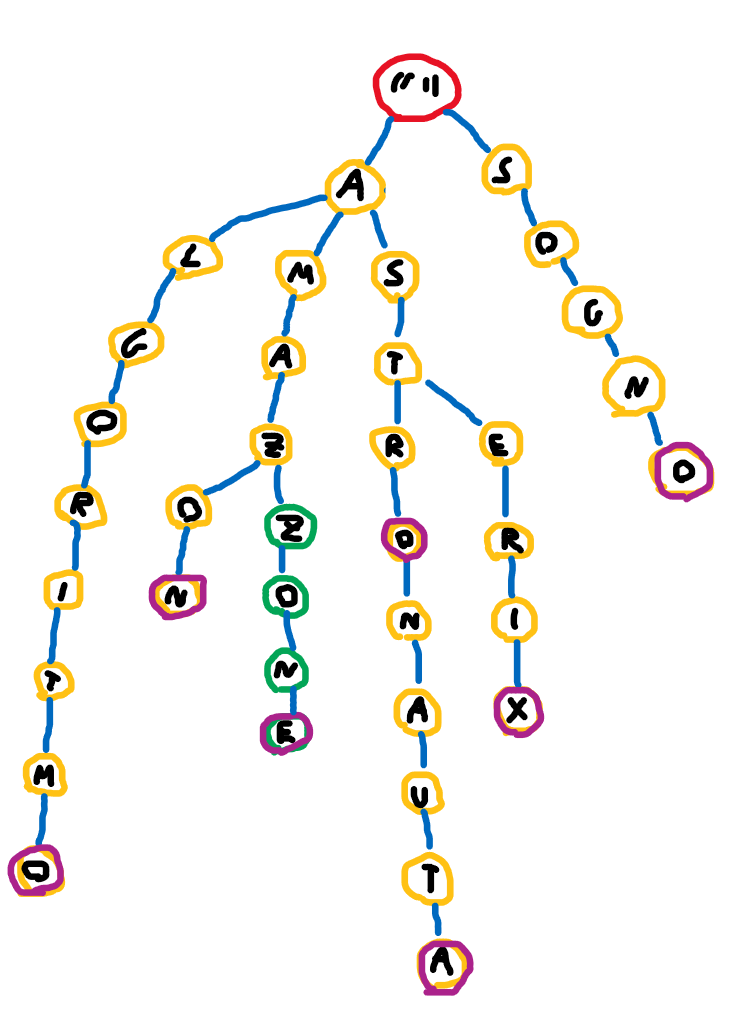
\includegraphics[width=8cm]{Images/trie dopo inserimento.png}
    \caption{Trie dopo l'inserimento di "Amazzone" e del prefix "Astro"}
    \label{fig:my_label}
\end{figure}

\clearpage

\subsubsection{Ricerca}
In questo paragrafo, verrà mostrato quanto è semplice e veloce recuperare una parola da un Trie, e perché è necessario mantenere un valore (o un booleano) come segnale di fine stringa, e come verrà utilizzato.

Supponendo che la parola da recuperare sia la nuova parola inserita, ovvero \textbf{Amazzone}, descriviamo i passaggi per ricercare la stringa:

\begin{itemize}
    
    \item A partire dalla radice, che ricordiamo essere la stringa vuota, cerchiamo tra i suoi link se è presente un riferimento alla lettera \textbf{A}.
    
    \item Non essendo \textbf{NULL}, sappiamo che il Trie contiene la lettera \textbf{A}. Continuando attraverso questo ramo, scendiamo giù, scandendo tutte le lettere che compongono la parola per trovare i link alle lettere successive. Per la precisione, verranno attraversati i seguenti nodi: \textbf{A - M - A - Z - Z - O - N - E}.
    
    \item Raggiunto l'ultimo nodo della parola (\textbf{E}), controlliamo il contenuto del valore da esso mantenuto. Esso contiene \textbf{25} (diverso da \textbf{NULL}), che rappresenta la fine della stringa. 
    
    Abbiamo recuperato (re\textbf{trie}ved) la parola \textbf{Amazzone}! Questo equivale ad un \textbf{Search Hit}, in quanto possiamo ritornare un valore per la chiave ricercata.
    
\end{itemize}

Ma cosa succederebbe se volessimo ricercare una parola che non esiste, come una sottostringa di \textbf{Amazzone}, per esempio \textbf{"Amaz"}? Come facciamo a capire che tale parola non è presente nel Trie?

\clearpage

Seguendo il procedimento della ricerca di una parola in un Trie:

\begin{itemize}
    
    \item Sempre a partire dalla radice, scorriamo i link \textbf{A - M - A - Z}.
    
    \item Raggiunto l'ultimo nodo della parola ricercata (\textbf{Z}), controlliamo il suo valore.
    
    \item Ci accorgiamo che il suo valore è \textbf{NULL}. Ciò equivale ad un \textbf{Search Miss}, in quanto non è possibile ottenere un valore dalla parola ricercata. Questo significa che la parola \textbf{Amaz} non esiste nel nostro Trie.
    
\end{itemize}

\textbf{\underline{Osservazione}}

Possiamo notare che, se volessimo aggiungere la parola \textbf{Amaz} nel nostro Trie, basterebbe scorrere fino all'ultimo nodo \textbf{Z} e settare un valore ad esso! Non sarà necessario allocare altro spazio per i nodi, in quanto i nodi \textbf{A - M - A - Z} sono gia stati creati nell'inserimento delle due parole \textbf{Amazon} e \textbf{Amazzone}. 

\begin{figure}[ht!]
    \centering
    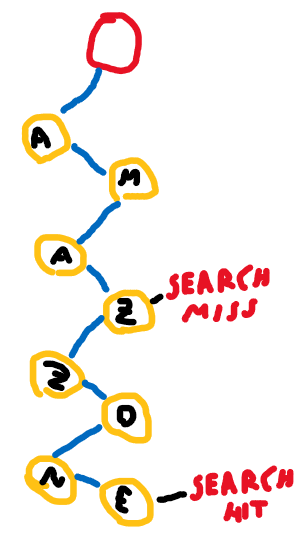
\includegraphics[width=4cm]{Images/ricerca.png}
    \caption{Esempio ricerca "Amazzone"}
    \label{fig:my_label}
\end{figure}

\subsubsection{Cancellazione}
L'operazione di cancellazione è molto semplice e veloce. E' necessario verificare certe condizioni e il gioco è fatto!

I casi in cui si incorre durante la cancellazione in un Trie sono i seguenti:

\begin{enumerate}
    \item La chiave non è presente nel Trie. In questo caso il Trie non viene alterato.
    
    \item La chiave è \textbf{unica}. Non sono presenti \textbf{prefissi} (chiavi che sono sotto-stringhe della chiave da cancellare); la chiave stessa da eliminare non è prefisso di una chiave più lunga. \textbf{Possiamo cancellare tutti i nodi}.
    
    \item La chiave è \textbf{prefisso} di una chiave più lunga. Si setta semplicemente il suo valore a \textbf{NULL}, rimuovendola logicamente.
    
    \item La chiave è presente nel Trie, ma è presente almeno una parola come \textbf{prefisso} della chiave da cancellare. A partire dall'ultimo nodo componente la chiave vittima, vengono cancellati i nodi fino ad arrivare al primo nodo che compone la chiave \textbf{prefisso} più lunga, che non dovranno essere cancellati.
\end{enumerate}

Analizziamo ogni caso di una cancellazione utilizzando le seguenti parole: \textbf{Algo}, \textbf{Sogno}, \textbf{Astro}, \textbf{Astronauta}.

\clearpage

\textbf{\underline{Caso 1: Algo}}

\vspace{5mm}
Questa parola permette di analizzare il primo caso: la chiave non è presente nel Trie.
Effettuiamo la ricerca della chiave. Attraversiamo i seguenti nodi: \textbf{A - L - G - O}, tutti presenti grazie alla parola pre-esistente \textbf{Algoritmo}.
Arrivato all'ultimo nodo \textbf{O}, controlliamo il suo valore. Quest'ultimo è \textbf{NULL}. Ciò significa che la chiave \textbf{Algo} non è presente nel Trie. Usciamo dalla procedura, senza alterare la struttura.

\vspace{5mm}

\textbf{\underline{Caso 2: Sogno}}

\vspace{5mm}
Siamo nel secondo caso: la chiave è unica, non sono presenti prefissi e la chiave stessa non è un prefisso.
Ricerchiamo la chiave. Percorriamo i seguenti nodi: \textbf{S - O - G - N - O}. L'ultimo nodo ha un valore diverso da \textbf{NULL}, quindi è presente nel Trie. 
Prima di tutto, settiamo il valore a \textbf{NULL}. Dopodiché, controlliamo se i suoi riferimenti sono anche essi a \textbf{NULL}. Se sono tutti vuoti, vuol dire che non sono presenti altre parole o~ramificazioni sotto la chiave, e sarà possibile cancellare i nodi. Incominciamo ad eliminare un nodo alla volta (in \textbf{Bottom-up}), fin quando non incontriamo un nodo il cui valore è diverso da \textbf{NULL} (che indica che è presente un \textbf{prefisso} della chiave che vogliamo cancellare). Essendo nel secondo caso, dove la chiave da eliminare è unica, risalendo il ramo non troveremo alcun prefisso, e tutti i nodi della parola \textbf{Sogno} verranno eliminati.

\clearpage

\textbf{\underline{Caso 3: Astro}}

\vspace{5mm}
Essa è prefisso della chiave \textbf{Astronauta}. Come nei casi precedenti, effettuiamo la ricerca del valore di \textbf{Astro}. Essendo diverso da \textbf{NULL}, esso è presente nella struttura. Controlliamo i riferimenti nell'ultimo nodo \textbf{O}, e ci accorgiamo che è presente un riferimento ad un nodo rappresentante la lettera \textbf{N}, appartentente alla parola \textbf{Astronauta}. In questo caso non possiamo cancellare alcun nodo, altrimenti non sarà più possibile recuperare la parola \textbf{Astronauta}. L'unico modo per rimuovere la parola \textbf{Astro} dal Trie è farlo logicamente settando il suo valore a \textbf{NULL}.

\vspace{5mm}

\textbf{\underline{Caso 4: Astronauta}}

\vspace{5mm}
L'ultimo caso è dovuto alla presenza di un prefisso all'interno della parola \textbf{Astronauta}, ovvero \textbf{Astro}. Dovremo stare attenti a non cancellare alcun nodo che componga quest'ultimo. Ipotizziamo che la cancellazione di \textbf{Astronauta} venga effettuata prima della cancellazione di \textbf{Astro}. Effettuiamo la ricerca del valore di \textbf{Astronauta}. Raggiunto l'ultimo nodo \textbf{A}, verifichiamo che non ci siano altri riferimenti. Essi sono tutti vuoti, quindi possiamo procedere in bottom-up alla rimozione dei nodi. Ma essendoci il prefisso \textbf{Astro} di mezzo, la procedura dovrà fermarsi una volta scoperto che il nodo \textbf{O} presenta un valore diverso da \textbf{NULL}.

\clearpage

\begin{figure}
    \centering
    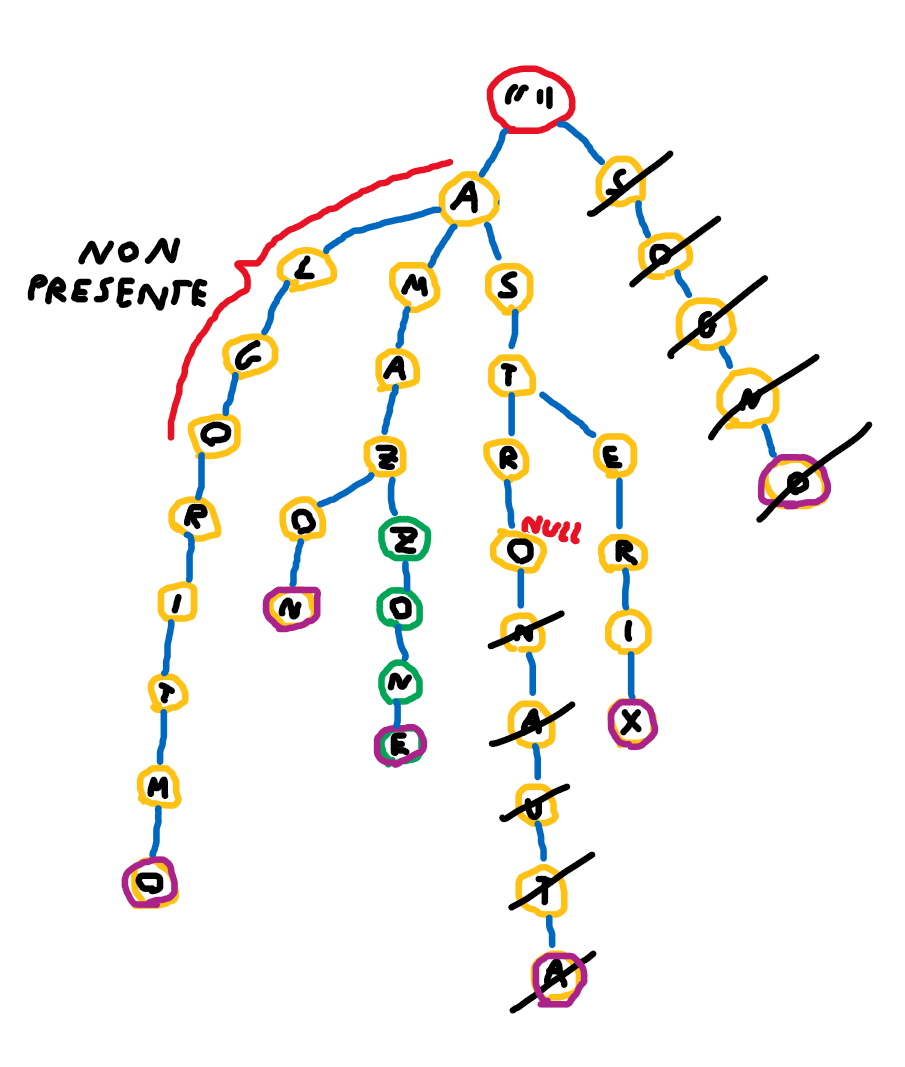
\includegraphics[width=10cm]{Images/dopo cancellazione.png}
    \caption{Trie dopo le cancellazioni}
    \label{fig:my_label}
\end{figure}

\clearpage

\subsection{Complessità}
Analizziamo le complessità di creazione di un Trie, insieme a quelle delle operazioni di inserimento, ricerca e cancellazione.

\begin{table}[th!]
    \centering
    \begin{tabular}{|c|c|}
    \hline
        \textbf{Operazione} & \textbf{Caso pessimo} \\
    \hline
        Creazione & O(m * n) \\ 
    \hline
        Inserimento & O(k) \\
    \hline
        Ricerca & O(k) \\
    \hline
        Cancellazione & O(k) \\
    \hline
    \end{tabular}
    \caption{Complessità Trie}
    \label{tab:my_label}
\end{table}

\begin{itemize}
    \item \textbf{Creazione}: la complessità spaziale di un Trie è direttamente proporzionale al numero di parole/chiavi che il Trie contiene. Sia \textbf{m} la lunghezza della parola più lunga nel Trie, e sia \textbf{n} il numero di parole contenute in esso, la complessità per la creazione di un Trie è: \textbf{O(m * n)}. Questo perché, se il Trie è vuoto, dovremo inizializzare un nodo per ogni lettera della stringa da inserire, in tempo costante. Questa operazione è ripetuta nel caso peggiore \textbf{m} volte, dove \textbf{m} è la lunghezza della stringa più lunga. Il tutto, ripetuto \textbf{n} volte, ovvero il numero di parole da inserire nel Trie.
    
    \item \textbf{Inserimento, ricerca, cancellazione}: sia \textbf{k} la lunghezza della parola considerata, la complessità temporale di ognuna delle tre operazioni è: \textbf{O(k)}.
    \begin{itemize}
        \item \textbf{Inserimento}: nel caso peggiore, la radice non ha un riferimento alla prima lettera della parola da inserire. Verranno istanziati \textbf{k} nodi, ognuno in tempo \textbf{O(1)}. \textbf{O(k)}
        \item \textbf{Ricerca}: nel caso peggiore, la stringa che stiamo cercando è la più lunga nel Trie. Se la sua lunghezza è \textbf{k}, verranno effettuati \textbf{k} accessi. \textbf{O(k)}
        \item \textbf{Cancellazione}: nel caso peggiore, la stringa è unica (non ha prefissi e a sua volta non è prefisso di una parola). Raggiunto il \textbf{k-esimo} nodo, ad uno ad uno vengono eliminati in Bottom-Up. \textbf{O(k)}
    \end{itemize}
\end{itemize}

\subsection{Vantaggi e svantaggi: Trie vs hash Table}
Trie e tabelle hash sono tanto simili quanto diversi. Entrambi fanno uso di un array, ma lo fanno in modo diverso. La tabella hash usa un array insieme a liste collegate, mentre il Trie usa un array in combinazione con dei puntatori a nodi.

La differenza sostanziale è che un Trie non fa uso di \textbf{funzioni hash}. Questo perché ogni parola ha una sua ramificazione unica che permette di raggiungere il suo valore. Quindi, è impossibile che ci siano \textbf{collisioni}, come accade con le tabelle hash. 

Inoltre, ogni parola è inserita in ordine alfabetico. Sarà sufficiente utilizzare gli indici dell'array che rappresentano le lettere dell'alfabeto, per accedervi.

Il lato negativo di avere una struttura semplice e veloce è che molto spazio viene sprecato. Ogni volta che viene inserita una lettera, un array viene istanziato con 26 puntatori a \textbf{NULL}, che probabilmente non verranno utilizzati del tutto. 

Per fare un esempio, l'inserimento della parola inglese \textbf{"Honorificabilitudinitatibus"}, lunga 26 caratteri, istanzierà 26 (array) * 26 (lettere alfabeto anglosassone) puntatori a \textbf{NULL}. Molto probabilmente, non verranno create delle sotto-ramificazioni a partire da questa parola, quindi molti dei suoi puntatori (o tutti), non verranno utilizzati, sprecando tantissima memoria.

Nonostante questo svantaggio, ulteriori benefici favoriscono l'utilizzo di un Trie come struttura dati per mantenere un set di stringhe. 

Inizialmente, ovviamente, verrà fatto tanto lavoro nell'inserimento delle prime parole, dovendo istanziare un nuovo array per ogni lettera inserita. Ma più il Trie cresce in dimensioni, meno lavoro sarà necessario per aggiungere un valore al suo interno, in quanto i nodi saranno gia stati inizializzati con i loro valori e riferimenti.

Un ulteriore vantaggio è dovuto dal fatto che la dimensione dell'alfabeto scelto rimane costante nel tempo. Nel caso dell'alfabeto anglosassone, ogni volta che vogliamo inserire una nuova lettera, sappiamo già che sarà necessario solamente controllare 26 possibili indici di un array presente in un nodo.

\subsection{Quando utilizzare un Trie}
La struttura \textbf{Trie} ha delle applicazioni particolari e molto interessanti. Quello più conosciuto, in quanto utilizzato tutti i giorni, è l'\textbf{auto-completamento}. Utilizzando il motore di ricerca Google, inserendo due/tre lettere, verranno proposte diverse parole che iniziano per quelle lettere che abbiamo inserito. Questo perché, una volta inserite le lettere, molti rami vengono tagliati, riducendo la dimensione dell'albero delle possibili parole, permettendo una facile enumerazione di quest'ultime. Ogni parola, come è gia stato descritto, può mantenere dei valori. Essi, oltre a rappresentare la fine della stringa, potrebbero essere scelti per indicare la popolarità di una parola, in modo tale che venga proposta una parola rispetto ad un'altra.

Ulteriori utilizzi di un Trie sono gli \textbf{algoritmi di matching} per l'implementazione di \textbf{spell checker}, oppure per implementare algorimti di \textbf{matching delle stringhe}.

Infine, un ulteriore utilizzo può essere quello dell'\textbf{ordinamento}. Un attraversamento \textbf{Pre-order} dell'albero darà come risultato un output di ordine crescente.

\subsection{Passare ad un altro alfabeto}
Fino ad ora abbiamo descritto il Trie facendo uso dell'alfabeto anglosassone. Esso è composto da 26 lettere, quindi per ogni nodo viene istanziato un array di dimensione 26. Ma se volessimo utilizzare la struttura, cosi per come l'abbiamo definita, in un'altra lingua, per esempio il \textbf{Cinese}? Sarà necessario modificare l'intero codice? Dipende dall'alfabeto. 

Partiamo con il presupposto che abbiamo consegnato il codice in versione inglese ad un'azienda cinese che vuole implementare un suo motore di ricerca con auto-completamento. Come è giusto che sia, tale azienda vorrebbe che le parole contenute nel Trie fossero in cinese. L'alfabeto cinese è composto da \textbf{21 lettere} (non vengono usate le lettere: j, k, w, x, y). Un numero inferiore rispetto all'alfabeto anglosassone. Sarà necessario modificare l'intera struttura per adattare il Trie all'alfabeto cinese? 

Potremmo mantenere la struttura in versione inglese (con array da 26 lettere), consapevoli del fatto che 5 lettere non verranno utilizzati, in quanto l'alfabeto cinese è composto da 21 lettere (incrementando lo spreco di memoria). Ma c'è un ulteriore problema: come ottenere l'indice associato ad una determinata lettera. Nella versione anglosassone, ogni lettera (in ASCII) è rappresentabile con \textbf{un byte} (\textbf{8 bit}). Risulta semplice estrarre dal carattere il suo indice: basta sottrarre al carattere considerato il carattere \textbf{'a'} (verrà effettuata una sottrazione bit a bit, che ci da come risultato un intero di 8 bit corrispondente all'indice). per fare un esempio: 
\begin{itemize}
    \item \textbf{'c' - 'a'} = \textbf{1100011 - 1100001} = \textbf{0000010} = \textbf{2} 
\end{itemize}

Purtroppo questo non è possibile con l'alfabeto cinese. Ogni carattere è codificato in \textbf{UTF-8} (servono \textbf{3 byte} per rappresentare un carattere cinese). Come se non bastasse, l'alfabeto cinese non è ordinato come quello anglosassone. In ASCII, i caratteri minuscoli, rappresentati in decimale, hanno un ordine numerico: \textbf{a = 97}, \textbf{b = 98}, \textbf{c = 99}, etc. Ciò non accade con l'alfabeto cinese. Quindi, l'approccio utilizzato con la versione inglese del Trie non è applicabile con l'alfabeto cinese.

L'unico modo per costruite un \textbf{Trie cinese} è:
\begin{itemize}
    \item Usare la struttura dati \textbf{Map} al posto dell'array
    \item Ogni elemento in un \textbf{Map} è una coppia \textbf{["carattere cinese", puntatore]}.
\end{itemize}

Il funzionamento è lo stesso. Per chiarire le idee, verrà presentato un esempio con il Trie costruito in precedenza:
\begin{itemize}
    \item Cerco la parola \textbf{Astro}.
    \item A partire dalla radice, controllo se dentro la \textbf{mappa} sia presente l'elemento \textbf{A}. La lettera \textbf{A} è presente nella mappa della radice, e da essa riesco a ricavare il puntatore al nodo \textbf{A}. 
    \item Raggiunto il nodo \textbf{A}, cerco dentro la sua mappa l'elemento \textbf{S}. Lo trovo ed estraggo il puntatore al carattere successivo.
    \item E cosi via, fino a raggiungere il nodo \textbf{O}, dentro la quale trovo il valore di fine stringa.
\end{itemize}

Questo approccio è applicabile con l'alfabeto cinese, con le lettere cinesi al posto di quelle latine.

\vspace{5mm}
\textbf{\underline{Osservazione}}

Utilizzando le \textbf{mappe}, è possibile risparmiare tantissimo spazio. Infatti, la mappa all'interno di un nodo manterrà solamente i riferimenti ai nodi figli successivi necessari, senza allocare altro spazio inutile come accade con gli array. 


\section{Pseudocodice}

Adesso che è stata data una visione completa del Trie, del suo utilizzo e delle operazioni che si possono effettuare su di esso, in questa sezione verranno presentati gli pseudocodici delle seguenti operazioni: \textbf{GetNode} (per creare un nuovo nodo), \textbf{Insert}, \textbf{Search}, \textbf{Delete}.

\subsection{GetNode}
Ricordiamo che ogni nodo (corrispondente ad una lettera di una word) mantiene un array di riferimenti a nodi figlio, corrispondenti alle lettere successive che compongono la parola. Se una lettera (nodo) di una parola che sta per essere inserita non è presente, è necessario crearlo con \textbf{GetNode}:

\vspace{5mm}
\begin{algorithm}[H]
\SetAlgoLined
  \textbf{Function getNode()}\\
  $node \leftarrow new\;TrieNode$\;
  $node.value \leftarrow NULL$\;
  \For{$i \leftarrow 0$ \KwTo $ALPHABET\_SIZE$}{
  $node.children[i] \leftarrow NULL$\;
  }
  \KwRet{$node$}\;
\caption{Creazione di un nuovo nodo}
\end{algorithm}

\clearpage

\subsection{Insert}
Partendo dalla radice, attraversiamo l'abero verso il basso, creando solamente i nodi mancanti. Raggiunto l'ultimo nodo, settiamo il suo valore diversamente da \textbf{NULL}.

\vspace{5mm}
\begin{algorithm}[H]
\SetAlgoLined
  \textbf{Procedure Insert(trie, key, value)}\\
  $node \leftarrow trie.root$\;
  \For{$i \leftarrow 0$ \KwTo $key.length$}{
    $index \leftarrow key[i] - {'a'} $\;
    \If{!node.children[index]}{
        $node.children[index] \leftarrow GetNode()$\;
    }
    $node \leftarrow node.children[index]$\;
  }
  $node.value \leftarrow value$\;
\caption{Inserimento di una nuova parola}
\end{algorithm}

\vspace{5mm}
\subsection{Search}
La funzione di ricerca è molto simile all'inserimento. A partire dalla radice, attraversiamo l'albero verso il basso. Se durante la discesa incontriamo un riferimento a \textbf{NULL} ancor prima di aver scansionato tutta la word che intendiamo cercare, significa che essa non è presente nel Trie. Se raggiungiamo l'ultimo nodo che compone la stringa, controlliamo se il suo valore è diverso da \textbf{NULL}. Se si, possiamo dire che la parola è presente nel Trie, altrimenti torniamo esito negativo.

\vspace{5mm}
\begin{algorithm}[H]
\SetAlgoLined
  \textbf{Function Search(trie, key)}\\
  \BlankLine
  $node \leftarrow trie.root$\;
  \BlankLine
  \For{$i \leftarrow 0$ \KwTo $key.length$}{
    $index \leftarrow key[i] - {'a'} $\;
    \BlankLine
    \If{!node.children[index]}{
        \KwRet{$FALSE$}\;
    }
    \BlankLine
    $node \leftarrow node.children[index]$\;
  }
  \BlankLine
  \eIf{$node \neq NULL$ $\&$ $node.value \neq NULL$}{
    \KwRet{$TRUE$}\;
  }
  {
    \KwRet{$FALSE$}\;
  }
\caption{Ricerca di una parola}
\end{algorithm}

\vspace{5mm}
\subsection{Remove}
La rimozione di una parola può essere implementata con una funzione ricorsiva. Questo perché, una volta raggiunto l'ultimo nodo componente la parola, dobbiamo risalire l'albero, eliminando un nodo alla volta (se possibile). Bisogna fare attenzione ai casi che si riscontrano durante la cancellazione, spiegati in \textbf{Pag.14}. 

\vspace{5mm}
\textbf{\underline{Caso base}}

I casi base sono due:
\begin{enumerate}
    \item La parola non è nel Trie (uno dei nodi sarà \textbf{NULL}).
    \item Abbiamo raggiunto l'ultimo carattere. In questo caso, controlliamo se il nodo contiene un valore di fine stringa diverso da \textbf{NULL}. In caso affermativo, lo settiamo a \textbf{NULL} per rimuoverlo logicamente dal set delle parole. Infine, controlliamo se tale nodo mantiene dei riferimenti a nodi figlo. Se sono tutti vuoti, possiamo procedere all'eliminazione del nodo. 
\end{enumerate}

\vspace{5mm}
\textbf{\underline{Passo ricorsivo}}

Ricaviamo l'indice del nodo figlio attraverso la stringa passata come parametro della funzione e chiamiamo ricorsivamente la funzione passando come parametri il Trie, la word da cancellare e la profondità dell'albero incrementata di uno, in modo tale da analizzare il carattere successivo. Dopo la chiamata ricorsiva, controlliamo se il nodo correntemente processato ha dei riferimenti a nodi figlio e se è segnato come fine stringa. Se entrambe le condizioni sono soddisfatte, vuol dire che ci sono rispettivamente altre ramificazioni che compongono altre word o che tale nodo appartiene ad un prefisso della stringa che vogliamo cancellare. In questo caso, non dobbiamo eliminare il nodo, o perderemo la possibilità di recuperare altre parole del set. Altrimenti, possiamo tranquillamente eliminarlo.

\vspace{5mm}
\begin{algorithm}[H]
\SetAlgoLined
  \textbf{Function Remove(root, key, depth)}\\
  \BlankLine
  \If{$!root$}{
    \KwRet{$NULL$}\;
  }
  \BlankLine
  \If{$depth = key.size$}{
    \If{$root.value \neq NULL$}{
        $root.value \leftarrow NULL$\;
    }
    \BlankLine
    \If{$isEmpty(root)$}{
        \textbf{Delete} root\;
        $root \leftarrow NULL$\;
    }
    \BlankLine
    \KwRet{$root$}\;
  }
  \BlankLine
  $index \leftarrow key[depth] - {'a'}$\;
  $root.children[index] \leftarrow Remove(root.children[index], key, depth + 1)$\;
  \BlankLine
  \If{$isEmpty(root)$ $\&$ $root.value = NULL$}{
    \textbf{Delete} root\;
    $root \leftarrow NULL$\;
  }
  \BlankLine
  \KwRet{$root$}\;
\caption{Eliminazione di una parola}
\end{algorithm}

\clearpage

\section{UML}
\begin{figure}[ht!]
    \centering
    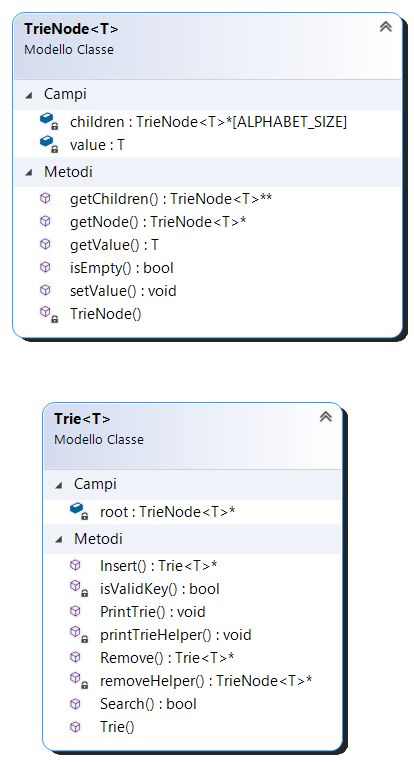
\includegraphics[width=8cm]{Images/ClassDiagram.png}
    \caption{Diagramma UML Trie}
    \label{fig:my_label}
\end{figure}

\clearpage

Come è possibile notare dal diagramma UML, il Trie è una struttura dati semplice, composta da due sole classi: una classe \textbf{TrieNode} corrispondente al singolo nodo che va a comporre un Trie, e la classe \textbf{Trie} stessa, composta da tanti TrieNode.

Ho deciso di utilizzare l'approccio dell'array come contenitore di riferimenti ai nodi figlio per la sua semplicità di utilizzo attraverso gli indici ordinati. Questo grazie al fatto che l'alfabeto utilizzato è ordinato ed è possibile ricavare da ogni lettera il suo indice di posizione (\textbf{A = 0, B = 1, ... , Z = 25}). Inoltre, l'aggiornamento dell'array è semplice: dato un nodo, se vogliamo aggiungere un nuovo riferimento all'i-esima lettera componente una parola, basta assegnare all'i-esima cella del suo array di riferimenti un nuovo nodo. Se vogliamo rimuovere quel riferimento, perché stiamo rimuovendo la parola a cui appartiene quel nodo, basta cancellare il nodo (con una \textbf{delete}) e assegnare \textbf{NULL} alla stessa i-esima cella.

Ad ogni inserimento, grazie agli array, la parola viene posizionata in ordine alfabetico in automatico, senza dover fare modifiche alla struttura.

\clearpage

\begin{thebibliography}{}
\bibitem{trie-description}  Frank Pfenning, 
                            "\emph{Lecture Notes on Tries}"
                             https://www.cs.cmu.edu/~fp/courses/15122-f10/lectures/18-tries.pdf

\bibitem{trie-complex}      Alex Chumbley, Agnishom Chattopadhyay, Karleigh Moore, and 3 others contributed.
                            "\emph{Tries}"
                            https://brilliant.org/wiki/tries/
                            
\bibitem{trie-1}            Alex Chumbley, Agnishom Chattopadhyay, Karleigh Moore, and 3 others contributed.
                            "\emph{Tries - Implementation}"
                             https://brilliant.org/wiki/tries/
                             
\bibitem{trie-1}            Daniel Ellard
                            "\emph{Tries - Implementation}"
                             http://ellard.org/dan/www/libsq/cb\_1998/c06.pdf
                             
\bibitem{trie-1}            geeksforgeeks.org
                            "\emph{Tries - Insert, Search, Remove}"
                             https://www.geeksforgeeks.org/trie-insert-and-search/?ref=rp
                             https://www.geeksforgeeks.org/trie-delete/?ref=rp
\end{thebibliography}

\end{document}
